\par \indent In the second half we would focus on behavioral loss aversion
analysis. We assessed behavioral sensitivity to gains and losses by fitting a
logistic regression to each participant's acceptability judgements collected 
during scanning, using the amount of gain, loss and the amount of the absolute 
diference between gain-loss combination as independent variables. On top of
this, we perform another logistic regression withought the third varialbe which 
is the difference between gain-loss pair. The purpose of doing the second
regression is to set up a comparison and see the to what extent does  having a 
weaker preference contribute to accept or reject the offer. Based on this 
analysis, we computed a measure of behavioral loss aversion \lambda as the ratio
of the (absolute) loss response to the gain response, which is yielded a median
\lambda = 1.882939 (range: 0.9505497 to 4.8956078) if the euclidean distance of 
gain/loss combination from the diagonal of the gamble matrix is not included, 
and a median of 1.861554 (range: 0.652284 to 5.345733) otherwise. Both
measurements are slightly different form the statistics stated in the paer that
lambda is a median of 1.93, ranging from 0.99 to 6.75. In general, this finding
is consistent with the observations that participants were, on average,
indifferent to gambles in which the potential gain was twice the amount of the 
potential loss. The estimated coefficients in front of gain, loss and 
with/without euclidean distance vastly vary across participants. 
    
\par \indent We first investigate individual behavioral reponse in decision 
making.The data set contains three runs for each subject, meanwhile, each run 
from each subject corresponds to one particular gain/loss combination. We take 
subject001 and run001 for example, the results are displayed below. We observe 
that with the additional parameter of euclidean distance, the p values are all 
considered
to be significant under the 0.05 significance level. The interpretation of \beta
is that is represents the increase in log-odds of the event that the subject 
takes the offer for a unit increase in one of the three conditions when all 
other explanatory variables are held constant. In other words, the e to the 
power of \beta denotes the factor by which the odds of sucess (success means
response accepts the gain/loss combination) change for a unit increase in one
of three explanatory variables (all other explanatory variables remaining 
unchanged). Undoubtedly, we obtain positive estimated coefficients for gain and
negative estimated coefficients for loss with the latter slightly smaller. 

\begin {figure}[!ht]
\centering
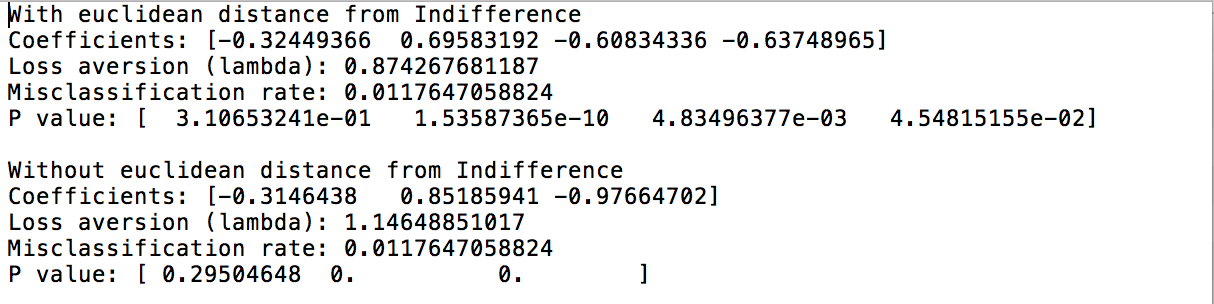
\includegraphics[width=120mm]{images/Sub001Run001.png}
\caption{Behavioral Logistic Regression Result for Subject001 Run001}
\label{fig:Logistic Regression}
\end{figure}

